\chapter{Números (2º Bimestre)}

\section{Números complexos}

Suponemos que existe un número $i$ tal que $i^2 = -1$ y consideramos el
conjunto de los complejos
$\mathbb{C} = \left\{ a + ib, a \in \mathbb{R}, b \in \mathbb{R} \right\}$.
Si $z = a + ib$, $a = \Re z$ es parte real y $b = \Im z$ la parte imaginaria.
Si $a = 0$,
$z$ es dicho número imaginario puro.
El conjugado de $z$ es $\bar{z} = a - i b$ y el módulo de $z$ es
${|z|} = \sqrt{a^2 + b^2}$. El complejo $z \neq 0$
puede ser representado en un plano de la manera siguiente:

\begin{center}
\begin{tikzpicture}
  \draw (0,0) node[left] {$0$} circle (2);
  \draw[style=dashed,color=gray] (0,0) circle (3);
  \draw[color=red] (0,0) -- (0.75,1.299038105676657) node[left] {$\rho$} --(1.5,2.598076211353315) node[right] {$z=a+ib$};
  \draw[->] (0,0) -- (4,0);
  \draw[->] (0,0) -- (0,4);
  \path (2,0) node[right] {$1$};
  \path (0,2) node[above] {$i$};
  \draw[style=dashed,color=blue] (1.5,2.598076211353315) -- (1.5,0) node[right] {$a$};
  \draw[style=dashed,color=blue] (1.5,2.598076211353315) -- (0,2.598076211353315) node[above] {$b$};
  \draw[color=green] (.5,0) arc (0:60:.5) node[right] {$\varphi$};
\end{tikzpicture}
\end{center}

If $z = a+ib$ y $z' = a'+ib'$, then we define the sum, difference and product
of complex numbers ``naturally'' by assuming that they are associative and
commutatitive and by using $i^2=-1$:
$$z + z' = {(a+a')} + i (b+b')$$
$$z - z' = {(a-a')} + i {(b-b')}$$
$$z \times z' = {a a'} + {i ab'} + {i a'b} + {(ib)(ib')} =
{(aa' - bb')} + i {(ab' + a'b)}$$

If $z \neq 0$, we note that $z \bar{z} = a^2 + b^2 + i {(ab - ab)} = {|z|}^2$
and so $z \frac{\bar{z}}{{|z|}^2} = 1$. Hence we define the inverse of
$z \neq 0$ by
$$z^{-1} = \frac{\bar{z}}{{|z|}^2}$$
and so the division of $z_1$ by $z_2\neq0$:
$$\frac{z_1}{z_2} = z_1 z_2^{-1}$$
%%
We then extended $\mathbb R$ to a set of complex numbers $\mathbb C$ with
very similar algebraic properties. The following exercise gives geometric
interpretation of $z_1+z_2$, $-z$, $z_1 \times z_2$, $\bar z$ (from which we
can calulate $z_1-z_2$, $z^{-1}$ and $\frac{z_1}{z_2}$). In $\mathbb R$, for
any $r$, there are two, one or no $s$ such that $s^2 = r$
($s=\pm\sqrt{r}$ if $r > 0$, $s=0$ if $r=0$ and no such $s$ if $r<0$). The
exercise shows that there in $\mathbb C$, any nonzero number has exactly
two square roots.

\subsection*{Exercício 1}

\begin{enumerate}
\item Muestrar que para cada número real $r \neq 0$, hay dos complejos
  $z_1 \neq z_2$ tal que $z_1^2 = z_2^2 = r$. ¿Que decir de esos números segun
  el signo de $r$?
\item En la representación gráfica, $\rho$ es el módulo de $z$ y el angulo
  $\varphi$ es llamado el argumento. Expresar $a, b$
  en función de $\rho$ y $\varphi$.
\item Cómo interpretar gráficamente la suma y conjugación de complejos?
\item What can you say about the $z$ and $-z$ on the graphical representation?
\item Recordar las formulas para el coseno y seno de la suma de dos ángulos.
  Si $z_1, z_2$ tienen módulos y argumentos $\rho_1, \varphi_1$ y
  $\rho_2, \varphi_2$, ¿Cómo se expresa el producto $z_1 \times z_2$ en función
  de esos parametros? ¿Cómo interpretar gráficamente el producto de dos
  complejos?
\item Deducir que para cada número real $r \neq 0$ sólo hay dos $z$ tal
  que $z^2 = r$ . ¿Que decir de $r=0$?
\end{enumerate}

\subsection*{Exercício 2}

Write these complex numbers in cartesian form $z=a+ib$.

\begin{enumerate}
\item ${(3i+8)}{(2i-3)}$
\item ${(i+1)}^3-5i+2$
\item $\overline{(6+i)}{(9i+8)}$
\item $\frac{1}{2i+3}$
\item $\frac{{(2+i)}^2}{3-7i}$
\end{enumerate}

\section{Equações polinomiais}

Let $n \geq 1$ and complex numbers $a_0, a_1, \dots, a_n$ such that $a_n\neq0$.
We consider the polynomial equation of degree $n$
%%
$$
a_n z^n + a_{n-1} z^{n-1} + \dots + a_1 z + a_0 = 0
$$
%%
where $z$ is an unknown complex number. Our goal is to find the solutions of
this equation.

If $n=1$, we can write $az+b = 0$ where $a\neq0$. Using the expression of
quotient of complex numbers from the previous section, we deduce that there is
a unique solution $z=-\frac{b}{a}$.

If $n=2$, we can write $a z^2 + b z + c = 0$. We can use the technique of the
2º bimestre of the 8ª série do Ensino Fundamental.
Se escrevermos $\Delta = b^2 - 4ac$ obtemos
%%
$$a z^2 + b z + c =
a \left( \left(z + \frac{a}{2b}\right)^2 - \frac{\Delta}{4a^2} \right)$$
%%
Se $\Delta = 0$, then by Exercício 1 a equação possui uma única solução
$z = -\frac{b}{2a}$.
Se $\Delta \neq 0$, then writing $\Delta$ in polar coordinates
$\rho={|\Delta|} \neq 0, \varphi_\Delta$ we can prove that there are actually two
solutions $\pm\delta$ where $|\delta| = \sqrt{\rho}$ and
$\varphi_\delta = \frac{\varphi_\Delta}{2}$
Then obtemos duas soluções
$$z_\pm = \frac{-b \pm \delta}{2a}$$
If $a,b,c \in \mathbb R$ these two solutions are given by
$\delta = \sqrt{\Delta}$ if $\Delta > 0$ and
$\delta = i \sqrt{|\Delta|}$ if $\Delta < 0$ (in that case $z_{-}=\overline{z_+}$).

It can be shown that any polynomial $P$ of degree $n$
can be factorized in $\mathbb C$:
$$
P(z) = {\sum_{i=0}^n a_i z^i} = a_n \prod_{j=1}^n \left(z-z_i\right)
$$
for some complex numbers $z_1, z_2, \dots, z_n$, called the roots of the
polynomial (these roots may not be pairwise distinct). As a consequence,
$z_1, z_2, \dots, z_n$ are the only possible solutions of the equation
$P(z) = 0$. If we know a root $r$ of $P$ and $Q = \frac{P}{{(z - r)}^{m_r}}$
where $m_r \geq 1$ is number of times $r$ appears in the factorization of $P$
then the equation $P(z) = 0$ is equivalent to $Q(z) = 0 \vee z = r$. This allows
to reduce the equation $P(z) = 0$ to an equation of lower degree $Q(z) = 0$.

If we expand $a_n \prod_{j=1}^n \left(z-z_i\right)$ and identify the coefficient
of degree $0 \leq i < n$ of the polynomial, we find the following relation
between the root and coefficient of the equation:
$$\sigma_{n-i} = \sum_{1 \leq j_1 < j_2 < \dots < j_{n-i} \leq n} \prod_{k=1}^{n-i} z_{j_k}a_i = {(-1)}^{n-i} \frac{a_n}{a_0} $$
In particular, the product and sum of roots can be expressed as
$$\sigma_1 = z_1+z_2+z_3\dots+z_n = -\frac{a_{n-1}}{a_n}$$
$$\sigma_n = z_1z_2z_3\dots z_n = {(-1)}^{n} \frac{a_0}{a_n}$$
For example if $az+b=0$ then $z_1 = -\frac{b}{a} = \sigma_1 = \sigma_n$.
Similarly, if $az^2+bz+c=0$ and $z_{\pm}$ are the
two solutions expressed above (maybe $\Delta = 0$ and so $z_- = z_+$) we have
$\sigma_1=z_+ + z_- = \frac{-b+\delta}{2a} + \frac{-b-\delta}{2a} = \frac{-b}{a}$ and
$\sigma_2=z_+ z_- = \frac{-b+\delta}{2a} \frac{-b-\delta}{2a} = \frac{b^2 - \Delta}{4a^2} = \frac{4ac}{4a^2} = \frac{c}{a}$.

According to Wikipedia, solutions to problems equivalent to the quadratic
equation were known as early as 2000 BC. The solutions of equations of degree
$n=3$ and $n=4$ using radicals were solved in the 15th/16th century by Italian
mathematicians.
Lagrange gave a nice interpretation of these methods that we sketch here
and in exercises 3 and 4. The polynomial expressions
of $\sigma_1, \sigma_2, \dots, \sigma_n$ are symmetric in $z_1, z_2, \dots, z_n$
that is they do not change after any permutation of these variables.
The polynomial $P = z_1 - z_2$ is not symmetric (we obtain $-P = z_2-z_1$ if we
exchange the variables $z_1,z_2$) but
$P^2 = {(z_1 - z_2)}^2 = z_1^2 + z_2^2 - 2z_1z_2$ is symmetric.
The key idea is that any symmetric polynomial in $z_1, z_2, \dots, z_n$ can be
expressed in function of $\sigma_1, \dots, \sigma_n$ and a fortiori in
function of the coefficients $a_0, a_1, \dots, a_n$ and so this can help
to solve the original equation. For example, if we consider the quadratic
equation $z^2 + bz + c = {(z-z_1)}{(z-z_2)} = 0$ then
$\sigma_1 = -{(z_1+z_2)} = -b$ and
$\sigma_2 = z_1z_2= c$. We can then express the symmetric polynomial
$P^2 = {(z_1-z_2)}^2$ as $P^2 = \sigma_1^2 - 4 \sigma_2 = b^2 - 4c = \Delta$.
The solutions are then
$z_1 = \frac{\sigma_1+P}{2}$ and $z_2 = \frac{\sigma_1-P}{2}$ where
$P$ is a square root of $\Delta$.

The Abel-Ruffini theorem states that there is no general solution
using elementary operations and radicals to polynomial equations of degree five
or higher with arbitrary coefficients. However, we can still handle some
specific cases such that $x^5 - 1 = 0$ (see exercise 5). Évariste Galois gave a
nice characterization of when a given polynomial equation can be solved
using elementary operations and radicals and this led to beautiful mathematical
theories. In particular Galois theory give a clear explaination of why a regular
polygon is constructible with rule and compass (see exercise 5).

\subsection*{Exercício 3}

\begin{enumerate}

\item Calculate $\left(-3\pm\sqrt{3}i\right)^3$.
\item Let $\rho = \frac{-1+i\sqrt{3}}{2}$. Calculate
  $\rho^2$ and $\rho^3$.
\item We consider the cubic equation
  $x^3-6x^2+11x-6= 0$
  with roots $x_1,x_2,x_3$. Recall the expressions of
  $\sigma_1,\sigma_2,\sigma_3$ in function of $x_1,x_2,x_3$.
\item Calculate $\sigma_1,\sigma_2,\sigma_3$ from the coefficient of the
  equation.
\item We let $y_1 = x_1+ \rho x_2 + \rho^2 x_3$ and
  $y_2 = x_1+ \rho^2 x_2 + \rho x_3$.
  Prove that $x_1 = \frac{y_1+y_2+\sigma_1}{3}$
\item Show that $y_1y_2$ and $y_1^3+y_2^3$
  are symmetric with respect to $x_1,x_2$.
\item Express $\sigma_1^2-3\sigma_2$,
  $2\sigma_1^3-9\sigma_1\sigma_2+27\sigma_3$,
  $y_1y_2$ and $y_1^3 + y_2^3$ in function of $x_1,x_2,x_3$. What do you notice?
\item Write ${(Y-y_1^3)}{(Y-y_2^3)}$ as a quadratic polynomial in $Y$ and
  deduce possible distinct values for $y_1, y_2$.
\item What are the solutions of the initial equation?
\end{enumerate}

\subsection*{Exercício 4}

\begin{enumerate}
\item We consider the cubic equation $y^3-\frac{5}{8} y^2 - \frac{205}{64} y
  + \frac{825}{512} = 0$. Verify that $\frac{15}{8}$ is a solution.
\item Deduce the two other solutions of the previous equation.
\item We consider the cuartic equation
  $x^4+\frac{5x^2}{8}+\frac{5x}{8}+\frac{205}{256}$.  Recall the expressions of
  $\sigma_1,\sigma_2,\sigma_3$ in function of $x_1,x_2,x_3$.
\item Calculate $\sigma_1,\sigma_2,\sigma_3, \sigma_4$
  from the coefficient of the equation and
  deduce that $x_4=\frac{{(x_1+x_4)} - {(x_1+x_2)} - {(x_1+x_3)}}{2}$.
\item We let $y_1=x_1x_2+x_3x_4$, $y_2=x_1x_3+x_2x_4$ and $y_3=x_1x_4+x_2x_3$.
  Show that ${(x_1+x_2)}^2 = -{(y_2+y_3)}$,
  ${(x_1+x_3)}^2 = -{(y_1+y_3)}$, ${(x_1+x_4)}^2 = -{(y_1+y_2)}$
\item Verify that $y_1+y_2+y_3=\sigma_2$,
  $y_1y_2+y_1y_3+y_2y_3=\sigma_1\sigma_3-4\sigma_4$,
  $y_1y_2y_3=\sigma_1^2\sigma_4-4\sigma_2\sigma_4+\sigma_3^2$.
\item Calculate the numeric values of coefficients $s_1,s_2,s_3$ such that
  ${(y-y_1)}{(y-y_2)}{(y-y_3)}=y^3 + s_1y^2+s_2y + s_3$? What are the
  values of $y_1,y_2,y_3$?
\item Show that the solutions $x_1,x_2,x_3,x_4$ of the cuartic equation are
  solutions to a system of the form
  $$
  \left\{
  \begin{gathered}
    x_1+x_2=-\epsilon_1\frac{\sqrt{5}}{2} \\
    x_1+x_3=-\epsilon_2\frac{i}{2}\sqrt{5-2\sqrt{5}} \\
    x_1+x_4=\epsilon_3\frac{i}{2}\sqrt{5+2\sqrt{5}} \\
    x_4=\frac{{(x_1+x_4)} - {(x_1+x_2)} - {(x_1+x_3)}}{2}
  \end{gathered}
  \right.
  $$
  for some $\epsilon_1,\epsilon_2,\epsilon_3 \in \{ -1, 1 \}$.
\item Deduce that the solutions of the cuartic equation are of the form
    $$x=\epsilon_1\frac{\sqrt{5}}{4}+
    \frac{i}{4} \left(\epsilon_2 \sqrt{5-2\sqrt{5}}+
    \epsilon_3 \sqrt{5+2\sqrt{5}} \right)$$
  for some $\epsilon_1,\epsilon_2,\epsilon_3 \in \{ -1, 1 \}$.
\item Show that for each value of $\epsilon_1,\epsilon_2,\epsilon_3$
  then at least one of $(\epsilon_1,\epsilon_2,\epsilon_3)$ or
  $(-\epsilon_1,-\epsilon_2,-\epsilon_3)$ does not correspond to a solution.
  Is it expected?
\end{enumerate}

\subsection*{Exercício 5}

We consider the equation $x^5-1=0$.

\begin{enumerate}
\item Find an obvious solution $x_0$.
\item Factorize $x^5-1$ as ${(x-x_0)}Q$ where $Q$ is a cuartic polynomial.
\item Simplify the expression $Q(y-\frac{1}{4})$.
\item Using Exercício 4, deduce that the solutions $x \neq x_0$ are of the form
    $$x=\frac{\epsilon_1\sqrt{5} - 1}{4}+
    \frac{i}{4} \left(\epsilon_2 \sqrt{5-2\sqrt{5}}+
    \epsilon_3 \sqrt{5+2\sqrt{5}} \right)$$
  for some $\epsilon_1,\epsilon_2,\epsilon_3 \in \{ -1, 1 \}$.
\item We now consider the complex numbers $x_k$ of module $\rho = 1$ and
  argument $\varphi = \frac{2 \pi k}{5}$ for $k=1,2,3,4$.
  Draw $x_0,x_1,x_2,x_3,x_4$ on the complex plan.
\item Use the geometric interpretation of the product of complex numbers
  (exercício 1) to calculate $x_k^5$ for
  $k=1,2,3,4$. Deduce that these $x_k$ are the remaining solutions of the
  equation.
\item What are the expression of the real and imaginary parts of $x_k$
  for $k=1,2,3,4$.
\item By comparing the real and imaginary parts, deduce the expression of the
  solutions $x_k$'s using radicals.
\item Compare with Exercício 7 of the 3º bimestre of the
  8ª série do Ensino Fundamental.
\end{enumerate}

\section{Solução do Exercícios}

\subsection*{Exercício 1}

\begin{enumerate}
\item Si $r > 0$ ya sabemos que $z_1 = -\sqrt{r}$ y $z_2 = \sqrt{r}$ convienen.
  Si $r < 0$, notamos que $z_1 = -i\sqrt{r}$ y $z_2 = i\sqrt{r}$ convienen
  tambíen porque $i^2 = -1$. Si $r > 0$ $z_1,z_2$ son reales y si $r < 0$,
  esos son imaginario puro.
\item $a = \rho {\cos(\varphi)}$, $b = \rho {\sin(\varphi)}$
\item La suma y resta se intepretan como suma de vectores. La conjucación como la simetria en el eje $X$.
\item $-z$ is the symmetric of $z$ with respect to the origin.
\item $z_1 z_2 = {\rho_1 \rho_2} \left({\cos(\varphi_1 + \varphi_2)} + i
  {\sin(\varphi_1 + \varphi_2)} \right)$. Entonces el módulo del producto es el
  producto de los modulos y el argumento del producto es la suma de los argumentos.
\item Si $z^2 = r$ y tenemos ${|z|}^2 = {|r|}$ y $2 \varphi \equiv 0 \mod 360°$ ($r > 0$) o $2 \varphi \equiv 180 \mod 360°$ ($r < 0$).
  Entonces $|z| = \sqrt{|r|}$ y $\varphi \equiv 0, 180 \mod 360°$ ($r > 0$)
  o $\varphi \equiv 90, 270 \mod 360°$ ($r < 0$), y esos son los soluciones
  encontradas arriba. Si $z \neq 0$, ${|z|} \neq 0$ y ${|z^2|} =
  {|z|}^2 \neq 0$. Entonces el único complejo tal que $z^2 = 0$ es $z = 0$.
\end{enumerate}

\subsection*{Exercício 2}

\begin{enumerate}
\item $-30+7i$
\item $-3i$
\item $57+46i$
\item $\frac{3-2i}{13}$
\item $\frac{-11+27i}{34}$
\end{enumerate}

\subsection*{Exercício 3}

\begin{enumerate}
\item We find $\pm 8i\sqrt{27}$
\item We find $\rho^2 = \frac{-1-i\sqrt{3}}{2} = -1 - \rho$ and $\rho^3 = 1$
\item $\sigma_1=x_1+x_2+x_3$, $\sigma_2=x_1x_2 + x_1x_3 + x_2x_3$ and
  $\sigma_3 = x_1 x_2 x_3$.
\item $\sigma_1=6$, $\sigma_2=11$ and $\sigma_3 = 6$.
\item Using the second question, we find
  $y_1+y_2=x_1-x_2-x_3=2x_1-x_2-x_3 = 3x_1 - \sigma_1$ so
  $x_1 = \frac{y_1+y_2+\sigma_1}{3}$.
\item Suppose we exchange $x_1,x_2$. The $y_1$ becomes
  $x_2+\rho x_1+\rho^2 x_3 = \rho y_2$ and
  $y_2$ becomes $x_2 + \rho^2 x_1 + \rho x_3 = \rho^2 y_1$.
  Then $y_1y_2$ becomes $\rho y_2 \rho^2 y_1 = y_1y_2$
  and $y_1^3+y_2^3$ becomes $\rho^3 y_2^3 + \rho^6 y_1^3 = y_1^3+y_2^3$.
  We have a similar result for other permutations of the root and so
  $y_1y_2$ and $y_1^3+y_2^3$ are symmetric.
\item We find
  $y_1y_2=\sigma_1^2-3\sigma_3=x_3^2+x_2^2+x_3^3-x_1x_2-x_1x_3-x_2x_3$ and
  $y_1^3+y_2^3 = 2\sigma_1^3-9\sigma_1\sigma_2+27\sigma_3 =
  2x_3^3+2x_2^3+2x_1^3-3x_2x_3^2-3x_1x_3^2-3x_2^2x_3-3x_1^2x_3-3x_1x_2^2-3x_1^2x_2+12x_1x_2x_3$. As stated, the symmetric polynomials $y_1y_2$ and
  $y_1^3+y_2^3$ can be expressed in function of $\sigma_1,\sigma_2,\sigma_3$.
\item We have ${(Y-y_1^3)}{(Y-y_2^3)} = Y^2 - {(y_1^3 + y_2^3)} Y + {(y_1y_2)}^3$.
  Using the previous question, this can be expressed in function of
  $\sigma_1,\sigma_2,\sigma_3$ and so in function of the coefficient of
  the cubic equation. We find
  $Y^2 + 27 = 0$ that is $y_1^3, y_2^3$ are $\pm i \sqrt{27}$.
  By the first question, possible values are
  $y_1,y_2 = \frac{-3\pm\sqrt{3}i}{2}$.
\item With the values chosen in the previous question, we obtain
  $x_1=\frac{y_1+y_1+\sigma_1}{3} = \frac{-3+6}{3} = 1$. We verify that indeed
  $1-6+11-6=0$. We can thus factorize the by $x-1$ and the remaining solutions
  are obtained from $x^2-5x+6 = 0$. We have $\Delta = 25-24=1$
  and solutions $\frac{5\pm1}{2}$. Hence the solutions of the initial equation
  are $x=1,2,3$.
\end{enumerate}

\subsection*{Exercício 4}

\begin{enumerate}
\item $\left(\frac{15}{8}\right)^3-\frac{5}{8} \left(\frac{15}{8}\right)^2 -
  \frac{205}{64} \left(\frac{15}{8}\right) + \frac{825}{512} =
  \frac{3375}{512} - \frac{1125}{512} - \frac{3075}{512} + \frac{825}{512} = 0$
\item We can factorize thus polynomial by $y - \frac{15}{8}$.
  The remaining solutions are thus obtained from $64y^2+80y-55 = 0$ which
  has solutions $y=\frac{-5\pm4\sqrt{5}}{8}$.
\item $\sigma_1 = x_1+x_2+x_3+x_4$,
  $\sigma_2 = x_1x_2+x_1x_3+x_1x_4+x_2x_3+x_2x_4+x_3x_4$,
  $\sigma_3 = x_1x_2x_3 + x_1x_2x_4 + x_1 x_3x_4 + x_2x_3x_4$
  and $\sigma_4=x_1x_2x_3x_4$.
\item $\sigma_1=0$, $\sigma_2=-\frac{5}{8}$, $\sigma_3=\frac{5}{8}$
  and $\sigma_4=-\frac{205}{256}$.
  Since $\sigma_1 = x_1+x_2+x_3+x_4=0$ we obtain
  $\frac{{(x_1+x_4)} - {(x_1+x_2)} - {(x_1+x_3)}}{2} =
  \frac{x_4-x_1-x_2-x_3}{2} = \frac{2x_4}{2} = x_4$.
\item We have $-{(x_1+x_2)} = x_3+x_4$ so
  $-{(x_1+x_2)}^2 = {(x_1+x_2)}{(x_3+x_4)}=x_1x_3+x_1x_4+x_2x_3+x_2x_4=y_2+y_3$
  Similarly for the others.
\item Express each of them in function of $x_1,x_2,x_3,x_4$.
  For example $y_1+y_2+y_3=x_1x_2+x_3x_4+x_1x_3+x_2x_4+x_1x_4+x_2x_3=\sigma_2$.
  Details of the two others are left to the student.
\item $s_1 = y_1+y_2+y_3 = \sigma_2 = -\frac{5}{8}$,
  $s_2 = -{(y_1y_2+y_1y_2+y_2y_3)}=4\sigma_4=-\frac{205}{256}$
  and $s_3=-y_1y_2y_3=4\sigma_2\sigma_4-\sigma_3^2=\frac{825}{512}$.
  This is the original cubic equation, so we can set
  $y_1=\frac{15}{8}$,
  $y_2=\frac{-5+4\sqrt{5}}{8}$ and $y_3=\frac{-5+4\sqrt{5}}{8}$.
\item
  The last equality has been proved in a previous question. For the others,
  ${(x_1+x_3)}^2 = -{(y_1+y_3)} = -\frac{5-2\sqrt{5}}{4} < 0$
  ${(x_1+x_2)}^2 = -{(y_2+y_3)} = \frac{5}{4} > 0$,
  and ${(x_1+x_4)}^2 = -{(y_1+y_2)} = -\frac{5+2\sqrt{5}}{4} < 0$. Each square
  gives two possible roots. So we finally obtain 8 possibilities
  for the triplet $(\epsilon_1,\epsilon_2,\epsilon_3)$.
\item Each choice of $(\epsilon_1,\epsilon_2,\epsilon_3)$ provides $4$ solutions
  after solving the linear system. However, many of these solutions are
  redundant and we can actually summarize them with the formula
    $$x=\epsilon_1\frac{\sqrt{5}}{4}+
    \frac{i}{4} \left(\epsilon_2 \sqrt{5-2\sqrt{5}}+
    \epsilon_3 \sqrt{5+2\sqrt{5}} \right)$$
  providing eight possibilities.
\item We note that if both $x$ and $-x$ are solutions, we would have
  $x^4+\frac{5x^2}{8}+\frac{5x}{8}+\frac{205}{256} = 0$ and
  ${(-x)}^4+\frac{5{(-x)}^2}{8}+\frac{5{(-x)}}{8}+\frac{205}{256} = 0$
  and so $x = 0$, a contradiction. Hence the previous expressions can
  only provide at most $4$ distinct solutions, which is expected since
  the equation is of degree $4$.
\end{enumerate}

\subsection*{Exercício 5}

\begin{enumerate}
\item Clearly, $1^5-1=0$ so $x_0=1$ is a solution.
\item We find $Q=x^4+x^3+x^2+x+1$
\item We find $Q(y-\frac{1}{4}) =
  y^4+\frac{5y^2}{8}+\frac{5y}{8}+\frac{205}{256}$
\item The possible solutions of $Q(y-\frac{1}{4}) = 0$ are given in Exercício 4.
  Then we obtain the solutions of $Q(x)=0$ via $x=y-\frac{1}{4}$.
\item They are on the unit circle since $\rho=1$ and placed on a regular
  pentagon since the argument is $\varphi = \frac{2 \pi k}{5}$ for
  $k=0,1,2,3,4$:

  \begin{center}
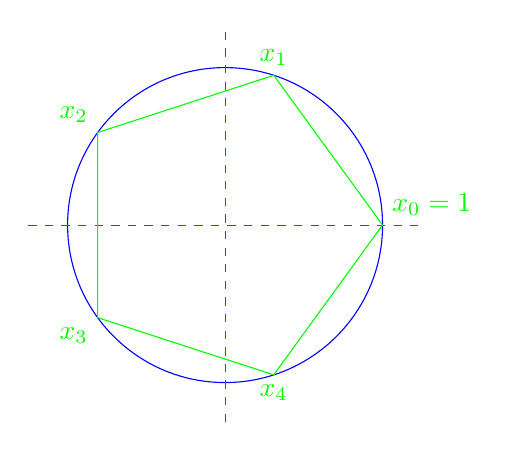
\begin{tikzpicture}[xscale=.5,yscale=.5]
  \draw (0,0) circle(4)[color=blue];
  \draw (-5,0) -- (5,0)[dashed,color=red];
  \draw (0,-5) -- (0,5)[dashed,color=red];
  \draw[color=green]
  (1.23606797749979,3.804226065180614)node[above]{$x_1$} --
  (-3.236067977499789,2.351141009169893)node[above left]{$x_2$} --
  (-3.23606797749979,-2.351141009169892)node[below left]{$x_3$} --
  (1.23606797749979,-3.804226065180614)node[below]{$x_4$} --
  (4, 0) node[above right]{$x_0=1$} -- cycle;

\end{tikzpicture}
\end{center}
\item The module of $x_k^5$ is the module of $x_k$ raised to power 5 that
  is $1^5 = 1$. The argument of $x_k^5$ is the five times the argument of $x_k$,
  that is $5 \frac{2\pi k}{5} = 2 k \pi \equiv 0 \mod 2\pi$. Hence
  $x_k^5=1$ and $x_k$ is solution of the equation.

\item $\cos\left(\frac{2\pi k}{5}\right)$ and
  $\sin\left(\frac{2\pi k}{5}\right)$.

\item From the schema (or formulas on $\cos$ and $\sin$) we see that
  $x_1$ and $x_4$ have the same positive real part and
  $x_2$ and $x_3$ have the same negative real part ; so the former is obtained
  for $\epsilon_1=1$ and the latter for $\epsilon_1=-1$.
  For the imaginary parts, we have $0 < \Im x_2 < \Im x_1$,
  $\Im x_3 = -\Im x_2$ and
  $\Im x_4 = -\Im x_1$. As a consequence, the imaginary parts of
  $x_1,x_2,x_3,x_4$ are respectively obtained for $(\epsilon_2,\epsilon_3)$
  being $(1,1)$, $(-1,1)$, $(1,-1)$ and $(-1,-1)$. Finally the solutions
  of $x^5-1=0$ are
%%
  $$x_0=1$$
  $$x_1=\frac{\sqrt{5} - 1}{4}+
  \frac{i}{4} \left(\sqrt{5-2\sqrt{5}}+\sqrt{5+2\sqrt{5}} \right)$$
  $$x_2=\frac{-\sqrt{5} - 1}{4}+
  \frac{i}{4} \left(-\sqrt{5-2\sqrt{5}}+\sqrt{5+2\sqrt{5}} \right)$$
  $$x_3=\frac{-\sqrt{5} - 1}{4}+
  \frac{i}{4} \left(\sqrt{5-2\sqrt{5}}-\sqrt{5+2\sqrt{5}} \right)$$
  $$x_4=\frac{\sqrt{5} - 1}{4}+
  \frac{i}{4} \left(-\sqrt{5-2\sqrt{5}}-\sqrt{5+2\sqrt{5}} \right)$$

\item We recover
  $\Re x_1 = \cos\left(\frac{2\pi}{5}\right) = \frac{\sqrt{5} - 1}{4}$.
  As seen in la 8ª série do Ensino Fundamental, this formula is enough to
  construct the regular pentagon using rule and compass.
  Note that more generally, constructing the regular $n$-gon
  using rule and compass is equivalent to
  expressing the all roots of the equation $X^n - 1 = 0$ using
  radicals (or at least one root of a polynomial $\Phi_n$ dividing $X^n - 1$
  and called a ``cyclotomic polynomial'').
  For example, the equilateral triangle ($n=3$), square ($n=4$),
  pentagon ($n=6$) and octogon ($n=8$) can be constructed since we know the
  how to express the value of trigonometric functions for the angles
  $\frac{\pi}{4}$, $\frac{\pi}{3}$, $\frac{\pi}{2}$ using radicals. However,
  one can show that the regular heptagon ($n=7$) is not constructible
  with rule and compass.
\end{enumerate}
